
\section{Introduction}
\label{sec:introduction}
In many edge communication systems, the receiver needs only information to execute a task, instead of reconstructing the transmitted message. This motivates the paradigm shift to task-oriented communications, where the performance is measured by task accuracy rather than bit error rate~\cite{beyond-bits,task-oriented}. A fundamentally practical class of tasks is binary decisions, such as membership tests and alarm rules. These can be interpreted as evaluating a Boolean function that represents the propositional formulae, providing a connection between communication and logical decision task~\cite{propositional-logic}.

Boolean function computation (BFC) via channels formalizes this setting~\cite{BFC}. Specifically, the transmitter owns a binary message $i$, while the receiver holds a function $f$ from a known family and aims to determine the function value $f(i)$. Importantly, the transmitter has no information about the selected function $f$, thus directly transmitting the result is unworkable. The primary problem in BFC via channel is the channel usage that can reliably compute a query without reconstructing the entire message.

Identification via channel~\cite{ID} is a special case of BFC, where the receiver determines whether the transmitter's message matches a particular message. Utilizing a randomized encoder, a doubly exponential number of messages in the channel blocklength can be reliably identified. Compared to the exponential growth in conventional transmission, task-oriented communication exhibits a fundamental difference. Recent work in~\cite{ID-task} also motivates identification through task-oriented communication in a joint identification and sensing scenario with noisy feedback.
Meanwhile, BFC covers a broader collection of binary decision tasks. Achievability and converse results for Boolean function families characterized by Hamming weights are established in~\cite{BFC-capacity}. Their results demonstrate a general relation between supported number of messages and channel use, depending on the the growth of Hamming weight with message length.

Reed-Solomon (RS) codes provide an explicit approach to code construction for identification via channel. Early works of \cite{CWC} established capacity-achieving identification codes based on concatenated constant-weight constructions. The RS tagging code construction for noiseless channel was proposed in \cite{RS-tagging}, and a concatenated RS tagging code was further developed in \cite{RS-performance} to achieve capacity. Subsequently, \cite{RS-implementation} implemented and evaluated on software-defined radios.

Reed-Solomon (RS) code provides an explicit tagging code construction for identification via channel. Specifically, the encoder randomly selects an index of a RS codeword and transmits this index together with the corresponding symbol. The error probability of such a code is guaranteed by the algebraic distance properties of RS code. The RS tagging code is first proposed for identification via noiseless channel in \cite{RS-tagging}. For noisy channels, a common and practical approach is to concatenated the noiseless RS tagging code with a conventional channel code~\cite{RS-tagging,ID-tutorial}.

In this paper, we develop the RS tagging code construction for BFC via channel. Over a binary noiseless channel, we first derive the upper bound for the error probability of the proposed code under finite-length. Built upon these bounds, we prove that an asymptotic computation rate of $1/2$ is achievable under our code construction. Then, we extend this construction to noisy channels by packing multiple tagging codes into one block and concatenating with a standard channel code. Both the finite-length and asymptotic performance are derived in terms of the effective channel use per BFC message. Numerical simulations are taken to demonstrate the effectiveness of the proposed code constructions.


\section{BFC Problem Formulation}
\label{sec:system_model}
Let $i\in\mathcal{I}_m:=\{0,1\}^m$ denote the binary message of length $m$ at the transmitter. The receiver selects a boolean function
\begin{equation}
    f:\mathcal{I}_m\to \{0,1\}
\end{equation}
from a family $\mathcal{F}_m$. Although the function family $\mathcal{F}_m$ is shared between both transmitter and receiver, the particular function $f$ is unknown to transmitter. Instead of estimating the complete message $i$, the receiver only needs to recover the value $f(i)$. Thus, the function $f$ represents the receiver's task.

Let $f^{-1}(1):=\{i\in\mathcal{I}_m:f(i)=1\}$ denote the pre-image of 1 under $f$. Then, the Hamming weight of $f$ is defined as
\begin{equation}
    S_f:=|f^{-1}(1)|.
\end{equation}
We primarily consider the class of constant weight boolean functions and the class of functions with Hamming weight no larger than $S$, denoted by
\begin{equation}
    \begin{split}
    \mathcal{F}_m(S) & :=\{f:\mathcal{I}_m\to \{0,1\}:S_f= S\},\\
    \mathcal{F}_m(\leq S) & :=\{f:\mathcal{I}_m\to \{0,1\}:S_f\leq S\}.
    \end{split}
\end{equation}
Particularly, computing the functions in $\mathcal{F}_m(1)$ is equivalent to the classic identification via channel problem \cite{ID}.

Consider a channel $W(\cdot|x^n)$ over space $\mathcal{Y}^n$ given input codeword $x^n\in\mathcal{X}^n$.
As defined in \cite{BFC}, an $(n,m,\mathcal{F}_m,\lambda_1,\lambda_2)$ BFC code consists of a stochastic encoder $Q_i$ on codeword space $\mathcal{X}^n$ for all $i\in\mathcal{I}_m$ and a decoding region $D_f\subseteq \mathcal{Y}^n$ for all $f\in \mathcal{F_m}$, such that the false-negative and false-positive are bounded by

\begin{align}
    P_{\rm FN}:=\max_{\substack{i,f:f(i)=1}}
    \sum_{x^n}Q_i(x^n)W(D_f^{\mathrm{c}}|x^n)
    &\leq \lambda_1, \label{equ:BFC_FN}\\
    P_{\rm FP}:=\max_{\substack{i,f:f(i)=0}}
    \sum_{x^n}Q_i(x^n)W(D_f|x^n)
    &\leq \lambda_2. \label{equ:BFC_FP}
\end{align}



Unlike conventional transmission, the maximal message length that can be reliably supported need not scale linearly with the channel use $n$ in the BFC problem \cite{BFC}. In fact, the scaling behavior of $m$ depends on the boolean function family. Therefore, we utilize a general scaling function to characterize the asymptotic performance.
\begin{definition}
\label{def:achievable}
Let $L:\mathbb{R}^{+}\times\mathbb{N}\to\mathbb{R}^{+}$
be a scaling function and $\{\mathcal{F}_m\}_{m\geq 1}$ be a sequence of boolean function families. An $(n,m,\mathcal{F}_m,\lambda_1,\lambda_2)$ BFC code supports finite-blocklength computation rate $R$ w.r.t. $L$ if
\begin{equation}
    \label{equ:finite_rate}
    m \geq L(R,n).
\end{equation}
\end{definition}
The function $L$ specifies the scaling of the supported message length, while $R$ parametrizes the computation rate at the given finite blocklength.
For example, $L(R,n)=nR$ represents the linear scaling in conventional Shannon transmission, whereas $L(R,n) = 2^{nR}$ represents the exponential scaling in identification via channel ($\mathcal{F}_m(1)$) \cite{ID}.
In Section~\ref{sec:noiseless}, we will characterize the scaling functions for different boolean function families under the propose RS tagging code construction.

The above formulations are independent of the particular channel model and can be generally applied to both the noiseless and noisy settings. In Section~\ref{sec:noiseless} we specialize the BFC problem to a binary noiseless channel and propose a RS code-based tagging code construction. In Section~\ref{sec:noisy}, we extend this code construction to a noisy channel by concatenating multiple tagging codewords with a channel code.

\section{BFC Codes over a noiseless channel}
\label{sec:noiseless}
\subsection{RS Tagging Code Construction}
\label{sec:tagging_code}
Let the size of finite space be $q=2^r$ and set $K=\lceil m/r\rceil$. The binary message $i$ of length $m$ is partitioned into $K$ consecutive $r$-bit blocks, with zeros appended if $r$ does not divide $m$. Each of these block can be interpreted as a symbol over $\F_q$. Therefore, the message can be denoted as $\bm z(i)=(z_0(i),\cdots,z_{K-1}(i))\in \F_q^K$, as shown in Fig.~\ref{fig:BFC_code}. Notably, when $r$ does not divide $m$ in a practical implementation, zero-padding will be applied. Now, we utilize an $(T,K)$ Reed-Solomon (RS) code over $\F_q$ to construct BFC code in a noiseless channel. Such a code outputs a length-$T$ codeword over $\F_q$ given a length-$K$ sequence over $\F_q$, requiring $1\leq K\leq T\leq q$. Specifically, each message $\bm z(i)$ is associated with a polynomial
\begin{equation}
    P_i(x):=
    \sum_{k=0}^{K-1}z_k(i)x^k.
\end{equation}
For all $N\in\N$, let $[N]:=\{1,\cdots,N\}$. The corresponding RS codeword is given by $\bm c(i)=(c_1(i),\cdots,c_T(i))$, where $c_\ell(i)=P_i(\alpha_\ell)$ and $(\alpha_\ell)_{\ell\in[T]}$ are distinct elements of $\F_q$.



The stochastic BFC encoder draws an index $U\sim\mathrm{Unif}[T]$ and selects the corresponding tag $c_U(i)$ to form a BFC codeword:
\begin{equation}
    A(i) = (U, c_U(i))\in \mathcal{A}:= [T]\times \F_q\subseteq\{0,1\}^{n_t}.
\end{equation}
Hence, the length of this tagging code is $n_t = \lceil\log T\rceil + r$. All logarithms are to base two. In a noiseless channel setting, $n_t$ is exactly the number of bits transmitted and the noiseless channel is characterized by $W(a'|a) = \1\{a'=a\}$ for all $a,a'\in\mathcal{A}$.

For a chosen boolean function $f$ at the receiver, we define the symbol-level decoding region at position $u$ as
\begin{equation}
    \label{equ:symbol_decoding_region}
    D_f(u):=\{c_u(j):j\in f^{-1}(1)\}.
\end{equation}
Consequently, the decoding region is given by
\begin{equation}
    D_f:=\{(u,v):u\in[T],\,v\in D_f(u)\}\subseteq \mathcal{A}.
\end{equation}
Given a received tagging code $a=(u,c_u)$, the decoder declares
\begin{equation}
    \hat f(a):=\1\{c_u \in D_f(u)\}.
\end{equation}
The code construction is summarized in Fig.~\ref{fig:BFC_code}.
\begin{figure}[htb]
    \centering
    \includegraphics[width=\columnwidth]{BFC_code_noiseless.pdf}
    \caption{RS tagging construction for BFC over a noiseless channel}
    \label{fig:BFC_code}
\end{figure}

\subsection{Finite-Length Results}
After formulating the code construction, we move on to its error analysis. Due to the tagging construction, the error analysis for BFC problem simply reduces to collision analysis between RS codeword symbols. In a noiseless channel, the RS symbol corresponding to a message is always contained in the decoding region at every position. Hence, a false-negative cannot occur. Whereas, a false-positive occurs when two messages have the same RS codeword symbol at the randomly selected index. Therefore, the performance of such a code construction is solely determined by the collision possibility of two distinct RS codeword. Utilizing the algebraic structure of RS code~\cite{RS-code}, we have the following finite-length error guarantee.
\begin{proposition}
\label{prop:finite_error}
For $0\leq S\leq 2^m$ and $n_t\geq 2$, consider the RS tagging construction in Section~\ref{sec:tagging_code}, based on a $(T,K)$ RS code over $\F_q$ satisfying $1\leq K\leq T\leq q$ and $n_t=\lceil\log T\rceil+r$. Then, the construction is an
\begin{equation}
    \left(
        n_t,m,\mathcal{F}_m(\leq S),
        0,
        \min\left\{1,\frac{S(K-1)}{T}\right\}
    \right)
\end{equation}
BFC code over the binary noiseless channel.
\end{proposition}


Proposition~\ref{prop:finite_error} gives a error guarantee for the RS tagging construction utilizing RS code parameters. The bound illustrates that a larger function Hamming weight $S$ leads to more collision and a larger $K$ carries more information bits at the cost of more collision. In contrast, increasing $T$ provides more randomization against choosing the collision position. For identification task ($S=1$), the worst case bound is tight, obtained directly by the algebraic property of RS code. For Boolean function families with higher Hamming weight, a union bound over $S$ messages in $f^{-1}(1)$ can be loose since their collisions may overlap.

Although Proposition~\ref{prop:finite_error} is expressed in terms of RS code parameters, these parameters are related to the blocklength $n_t$. Specifically, $n_t=\lceil\log T\rceil + r$ and $m=rK$, while RS feasibility requires $K\leq T\leq 2^r$.
Therefore, the error probability bound can be relaxed to $mS(m)/(rT)$. Minimizing this is equivalent to maximizing $(n_t-\lceil \log T\rceil)T$ with constraint $\lceil \log T\rceil\leq n_t-\lceil \log T\rceil$. Since this expression is non-decreasing with $\lceil \log T\rceil$, the optimal is achieved by
\begin{equation}
    r=\lceil n_t/2\rceil,\quad T=2^{\lfloor n_t/2\rfloor}.
\end{equation}
Substituting these parameters into Proposition~\ref{prop:finite_error} makes the dependence on $n_t$ explicit and yields the following finite blocklength tradeoff.

\begin{theorem}
    \label{thm:finite_E2}
    Let $S:\N\to\N$ be non-decreasing and define scaling function as
    \begin{equation}
        \label{equ:scaling_function}
        L_S(R,n):=\max\left\{m\in\N:mS(m)\leq\frac{n}{2}2^{nR}\right\}.
    \end{equation}
    For all $E_2\in(0,1/2)$ and $n_t\in\N$ with $n_t\geq 2$ for which the set in $L_S(1/2-E_2,n_t)$ is non-empty, set $r=\lceil n_t/2\rceil$, $T=2^{\lfloor n_t/2\rfloor}$, and $m=\min\{L_S(1/2-E_2,n_t),rT\}$. Then, the RS tagging construction gives an
    \begin{equation}
        \left(n_t, m, \mathcal{F}_m(\leq S(m)), 0, \min\left\{1,\sqrt{2}2^{-n_tE_2}\right\}\right)
    \end{equation}
    BFC code. If $L_S(1/2-E_2,n_t)\leq rT$, this code supports computation rate $1/2-E_2$ w.r.t. $L_S$. Otherwise, it supports rate $R$ satisfying $L_S(R,n_t)\leq rT$.
\end{theorem}

Based on the error exponent $E_2$, Theorem~\ref{thm:finite_E2} explicitly characterize the trade-off between error probability and the supported message length. Particularly, A larger $E_2$ yields a faster error decay rate, while reduces argument $1/2-E_2$ of scaling function, resulting in a smaller supported message length. For even $n_t$, the constraint $m\leq rT$ is inactive, and the false-positive probability can be improved to $2^{-n_tE_2}$.
Meanwhile, for odd $n_t$, the constraint is inactive for sufficiently large $n_t$, which leads to the asymptotic results in the following.


\subsection{Asymptotic Results}

Although our primary result is the finite-blocklength tradeoff in Theorem~\ref{thm:finite_E2}, its asymptotic performance also provides a concise benchmark and enables comparison with the existing BFC capacity results in \cite{BFC,BFC-capacity}. We first state the asymptotic notion utilized in this
\begin{definition}
    \label{def:asymptotic_rate}
    Let $L$ be a scaling function and $\{\mathcal{F}_m\}_{m\geq 1}$ a sequence of Boolean function families. A rate $R>0$ is asymptotically achievable for $\{\mathcal{F}_m\}_m$ w.r.t. $L$ if, for all $\lambda_1,\lambda_2,\eta>0$, and sufficiently large $n$, there exist an $m\in N$ and an $(n,m,\mathcal{F}_m,\lambda_1,\lambda_2)$ BFC code that supports finite-blocklength computation rate $R-\eta$ w.r.t. $L$.
\end{definition}

In the asymptotic regime, we focus on even blocklength. For odd blocklength $n_t$, appending one unused channel use does not change the asymptotic rate. Taking a fixed $E_2=\eta>0$ in Theorem~\ref{thm:finite_E2} yields the following asymptotic result.

\begin{corollary}
    \label{thm:general_asymptotic}
    Let $S:\mathbb{N}\to\mathbb{N}$ be non-decreasing. Then $1/2$ is an asymptotically achievable computation rate for $\mathcal{F}_m(\leq S(m))$ under the RS tagging construction w.r.t. $L_S$ in \eqref{equ:scaling_function}.
\end{corollary}



The established rate of $1/2$ reflects the equal allocation of channel uses to both index and tag. Crucially, the implicit definition for scaling function $L_S$ yields a unified result for all function families $\mathcal{F}_m(\leq S(m))$. To translate it into more interpretable expressions, we classify the function families by the growth rate of $S(m)$ w.r.t. the message length $m$, yielding explicit scaling functions.

\begin{corollary}
    \label{cor:weight_regimes}
    Let $S:\N\to\N$ be non-decreasing and $S^{\leftarrow}(x):=\max\{m\in\N:S(m)\leq x\}$. Under the RS tagging construction in Section~\ref{sec:tagging_code}, we have
    \begin{itemize}
        \item If $\frac{\log S(m)}{\log m}\to a$ for some $a\geq 0$ as $m\to\infty$, then $\frac{1}{2(1+a)}$ is an achievable rate w.r.t. $L_{\mathrm{small}}(R,n)=2^{Rn}$.
        \item If $\frac{\log S(m)}{\log m}\to \infty$ as $m\to\infty$, and $\frac{\log S(m)}{m}\leq \alpha$ for some $\alpha\in(0,1)$, then $\frac{1}{2}$ is an achievable rate w.r.t. $L_{\mathrm{medium}}(R,n)=S^{\leftarrow}(2^{Rn})$.
        \item If $\frac{\log S(m)}{m}\to 1$ as $m\to\infty$, then $\frac{1}{2}$ is an achievable rate w.r.t. $L_{\mathrm{large}}(R,n)=Rn$.
    \end{itemize}
\end{corollary}



Corollary~\ref{cor:weight_regimes} explicitly illustrates that the scaling function of BFC problem highly depends on the Boolean function Hamming weight. A polynomial growth $S(m)=m^a$ allows for an exponential scaling for the support message length. When $S(m)$ grows faster but remains sub-exponential, its inverse $S^{\leftarrow}$ sets the scaling. Finally, at exponential growth $S(m)=2^m$, the supported message length becomes linear in $n$, as in conventional transmission.

For a binary noiseless channel, the theoretical bounds in~\cite{BFC-capacity} gives a computation capacity $1$ when $a=0$ in the small-weight regime, a capacity in $[1/(1+2a),1/(1+a)]$ when $a>0$, a capacity in $[1/2,1]$ in the medium-weight regime, and capacity $1$ in the large-weight regime.
Accordingly, our explicit RS tagging construction achieves one half of the exact capacity when $a=0$ and in the large-weight regime. For $a>0$, its rate $1/[2(1+a)]$ is one half of the converse upper bound in~\cite{BFC-capacity}, whereas in the medium-weight regime its rate $1/2$ matches the general achievability lower bound.
Notably, the rate $1/2$ achieved by our RS tagging construction is not optimal in the large-weight regime, since transmitting the entire $m$-bit message achieves rate $1$ w.r.t. $L_{\rm large}$.


\subsection{Numerical Results}
\label{sec:noiseless_numerical}
We evaluate identification ($S=1$), the rank test
$f(i)=\1\{\operatorname{int}(i)\leq20\}$ ($S=21$), and the exact-threshold
test $f(i)=\1\{\|i\|_1=2\}$ ($S=\binom{m}{2}$). For
$n_t\in\{24,26,\ldots,40\}$ and $E_2=0.1$, we set $r=n_t/2$, $T=2^r$,
and $m=rK$, with the largest $K$ satisfying
$K S_{\rm up}(rK)\leq2^{n_t(1/2-E_2)}$, where $S_{\rm up}=S$ for
identification and rank, and $S_{\rm up}(m)=m^2/2$ is a conservative
envelope for the exact-threshold support. The finite rate is
$R_t=\log_2(m)/n_t$. For each setting, we sample $2{,}000$ negative
messages ($200$ for identification at $n_t=38,40$) and enumerate all $T$
RS positions, giving the exact conditional FP probability of each sampled
message; FN is zero by construction.

Fig.~\ref{fig:itw27_noiseless}(a) directly checks
Proposition~\ref{prop:finite_error}: every sampled FP probability is below
$B=S(K-1)/T$. At $n_t=40$, the sampled maxima are
$3.81\times10^{-6}$, $3.62\times10^{-5}$, and $7.04\times10^{-3}$ for
identification, rank, and exact threshold, respectively, versus bounds
$0.0625$, $0.0625$, and $0.0340$, showing that the uniform guarantee can be
conservative for these functions. Separately, $22$ tested arbitrary
supports attain $B$ exactly; this confirms tightness for those unrestricted
supports, not for the named rank and threshold functions.
Fig.~\ref{fig:itw27_noiseless}(b) deterministically evaluates the certified
design. With fixed $E_2=0.1$, the rates approach $0.4$
for constant weights and $2/15$ for $\beta=2$; with
$E_2(n_t)=n_t^{-1/2}$, the bound $2^{-\sqrt{n_t}}$ vanishes while the rates
approach the asymptotic benchmarks $1/2$ and $1/6$. Finite-length
prefactors explain values above a benchmark at small $n_t$.

\begin{figure}[t]
  \centering
  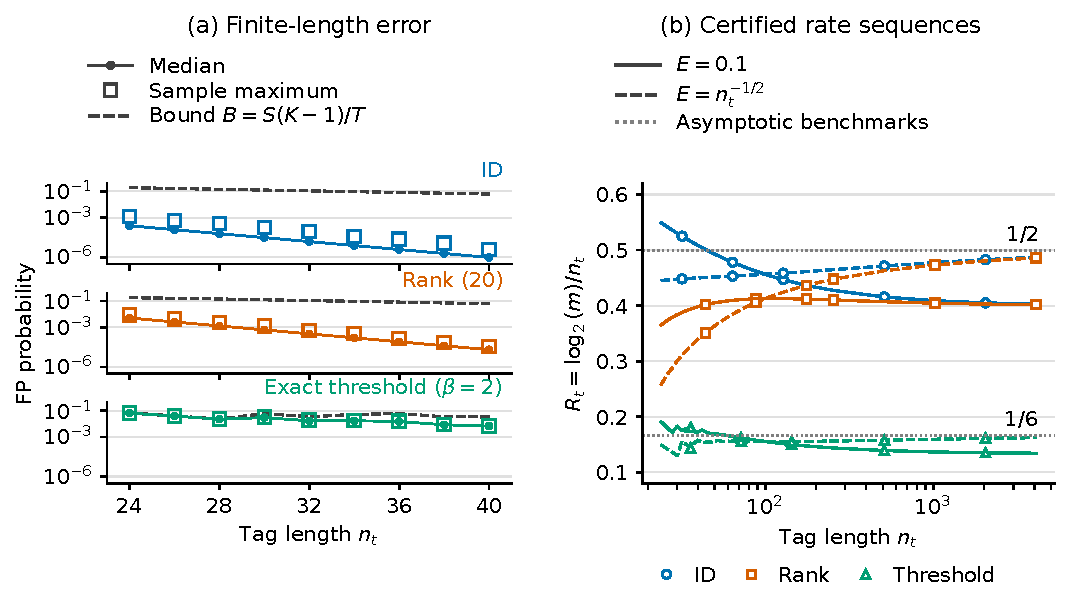
\includegraphics[width=\columnwidth]{itw2027/results/processed/figures/figure1_noiseless.pdf}
  \caption{Noiseless RS tagging: (a) sampled conditional FP probabilities and uniform bounds; (b) certified finite rates and asymptotic benchmarks.}
  \label{fig:itw27_noiseless}
\end{figure}




\section{Concatenated Extension to Noisy Channels}
\label{sec:noisy}
The RS tagging construction in Section~\ref{sec:tagging_code} gives a tagging codeword $A(i)=(U,c_U(i))$ with length $n_t=\lceil\log T + r\rceil$ bits. To transmit over a noisy channel, this codeword needs to be protected against channel distortions. A natural approach is concatenating this noiseless BFC code with a standard channel code \cite{RS-tagging}. However, this can be highly inefficient since $n_t$ is considerably smaller than the information block length of a practical modern channel code. Therefore, we pack several tagging codeword generated by independent messages into one information block and apply channel encoding.

The resulting construction acts as a separate source and channel code. The RS tagging code introduces the false-positive due to tag collision, whereas the channel decoding error may introduce additional error to tagging codeword. In the following, we first formally introduce the packed concatenated RS tagging code construction, then bound the error probability and demonstrate the asymptotic achievable rate.


\subsection{Packed Concatenated RS Tagging Code Concatenation}
\label{sec:packing_concatenation}
Consider a binary channel $W$ and a $(N_b,N_i,\xi)$ channel code with encoder $\phi_{\rm c}:\{0,1\}^{N_i}\to\mathcal{X}^{N_b}$ and decoder $\psi_{\rm c}:\mathcal{Y}^{N_b}\to\{0,1\}^{N_i}$, where $N_b$ denotes the block length, $N_i$ denotes the information length, and the maximal frame error rate is $\xi$. Thus channel code rate is $R_c = N_i/N_b$.


Each RS tagging codeword takes $n_t$ bits. For simplicity, we assume $n_t$ divides $N_i$. Hence, one information block can pack $G=N_i/n_t\in\N$ independent tagging codewords. In practical implementation, zero padding will be applied if $n_t$ does not divide $N_i$. Therefore, the effective channel use per BFC message is
\begin{equation}
    n_{\rm eff} = \frac{N_b}{G}=\frac{n_t}{R_c}.
\end{equation}
The quantity $N_b$ is the physical blocklength of the packed channel code, whereas $n_{\rm eff}=N_b/G$ is a normalization per BFC task.

For each slot $g\in[G]$, let the corresponding message denoted as $i_g\in\mathcal{I}_m$. The RS tagging encoder draws an index $U_g\overset{\rm i.i.d.}{\sim}{\rm Unif}[T]$ and generates codeword $A_g=(U_g,c_{U_g}(i_g))$. The binary representations of $(A_1,\cdots,A_G)$ are concatenated in a known order, resulting an $N_i$ bits information block $V\in\{0,1\}^{N_i}$. Then, the channel encoder transmits $X^{N_b}=\phi_{\rm c}(V)$.

Given the channel output $Y^{N_b}\sim W(\cdot|X^{N_b})$, the channel decoder computes $\psi_{\rm c}(Y^{N_b})$ and recovers $G$ tagging codewords $\hat A_g=(\hat U_g,\hat C_g)$, $g\in[G]$. For each slot, the receiver can select a function $f_g\in\mathcal{F}_m$. Utilizing the symbol-level decoding region $D_{f_g}$ defined in \eqref{equ:symbol_decoding_region}, the decision for slot $g$ is
\begin{equation}
    \hat f_g=\1\{\hat U_g\in[T], \hat C_g\in D_{f_g}(\hat U_g)\}.
\end{equation}
If an index $\hat U_g$ does not correspond to any element of $[T]$ due to channel distortion, the decoder declares zero. Note that choose $T = 2^t$ for some integer $t\leq r$, then the binary sequence $\hat U_g$ always correspond to one element in $[T]$.

\subsection{Finite-Length and Asymptotic Performance}
The packing construction changes the total channel uses, but the decision for each BFC message remains the same. For each slot utilizing the effective channel use $n_{\rm eff}$, an error arise either from an RS symbol collision or channel decoding error. Separating the error guarantee for noiseless RS construction with the channel code yields the following Proposition~\ref{prop:finite_error}.
\begin{proposition}
    \label{prop:noisy_finite_error}
    Consider the packed concatenated RS tagging code construction in Section~\ref{sec:packing_concatenation}, that concatenates the noiseless BFC code in Proposition~\ref{prop:finite_error} with an $(N_b,N_i,\xi)$ channel code. Then, the construction is an effective
    \begin{equation}
        \left(n_{\rm eff},m,\mathcal{F}_m(\leq S),\xi,\min\left\{1,\frac{S(K-1)}{T}+\xi\right\}\right)
    \end{equation}
    BFC code.
\end{proposition}
By an ``effective $(n_{\rm eff},m,\mathcal{F}_m,\lambda_1,\lambda_2)$ BFC code'' means that the code utilizes $N_b$ channel uses to simultaneously serve $G$ tasks, satisfying the BFC error guarantees for each task. Thus, it does not assert the existence of an ordinary BFC code whose physical blocklength is $n_{\rm eff}$.



Proposition~\ref{prop:noisy_finite_error} demonstrates that the noisy channel extension preserves the structure of the noiseless error probability bound. Given a correct channel decoding, the false-positive is exactly the same as noiseless channel scenario. A channel failure contributes an additional error probability $\xi$. The additive structure implies a separate source and channel coding framework. Notably, packing does not introduce a factor $G$ in the error analysis, having no affect the worst-case error of an individual task.

Consequently, the finite-length tradeoff developed for noiseless construction in Theorem~\ref{thm:finite_E2} can be reused in the noisy channel setting.
Particularly, since $n_t=R_cn_{\rm eff}$, the RS parameters can be expressed in terms of the effective channel use $n_{\rm eff}$. Together with the additional error $\xi$ contributed by channel code, we have the following finite-length result.
\begin{corollary}
    \label{cor:noisy_finite_E2}
    Define
    \begin{equation}
        \label{equ:noisy_scaling_function}
        L_{S,R_c}(R,n) := \max\left\{m\in\N:mS(m)\leq\frac{nR_c}{2}2^{nR}\right\}.
    \end{equation}
    Suppose $r$ and $T$ are chosen as in Theorem~\ref{thm:finite_E2}, and the channel code satisfies $\xi\leq 2^{-N_b E_{\rm ch}}\leq 1$, for some $E_{\rm ch}>0$
    For all $E_2\in (0,R_c/2)$, set $m=\min\{L_{S,R_c}(R_c/2-E_2,n_{\rm eff}),rT\}$, then the packed concatenated RS tagging construction gives an $(n_{\rm eff},m,\mathcal{F}_m(\leq S(m)),\lambda_1,\lambda_2)$ BFC code, where
    \begin{equation}
        \lambda_1 =2^{-N_b E_{\rm ch}},\quad \lambda_2 = \min\left\{1,\sqrt{2}2^{-n_{\rm eff}E_2} +\lambda_1\right\}.
    \end{equation}
    If $L_{S,R_c}(R_c/2-E_2,n_{\rm eff})\leq rT$, this code supports computation rate $R_c/2-E_2$ w.r.t. $L_{S,R_c}$. Otherwise, it supports rate $R$ satisfying $L_{S,R_c}(R,n_{\rm eff})\leq rT$.
\end{corollary}

Similar to Theorem~\ref{thm:finite_E2}, the error exponent $E_2$ provides a tradeoff between error and rate. The factor $R_c$ implies that only a fraction of the physical channel uses are available to carry RS tagging bits. Therefore, in the asymptotic regime, the achievable computation rate over the noisy channel is also scaled by the channel code rate. Formally, we have the following asymptotic result.

\begin{corollary}
    Under the assumptions of Corollary~\ref{cor:noisy_finite_E2}, for all fixed $R_c$ for which the channel decoding error vanishes asymptotically, $R_c/2$ is an achievable computation rate for $(\mathcal{F}_m(\leq S(m))$ under the packed concatenated RS tagging construction w.r.t. $L_{S,R_c}$.
\end{corollary}
Crucially, if a capacity-achieving sequence of channel codes is employed, the code construction achieves an asymptotic computation rate of $C/2$, where $C$ is the capacity of the underlying noisy channel.




\subsection{Numerical Results}
\label{sec:noisy_numerical}
We concatenate the tags with a rate-$1/2$ normal-frame DVB-S2 LDPC code
($N_b=64{,}800$, $N_i=32{,}400$), transmit BPSK over AWGN, and use
belief-propagation decoding with early termination and at most $50$
iterations. The sweep uses $E_b/N_0=0.5,0.6,\ldots,2.6$ dB and $2{,}500$
frames per point, where $E_b$ is normalized per occupied payload bit. A
fixed, balanced bank of positive and negative examples is reused across
SNRs for each function, so FP and FN are class-conditional; frames, rather
than packed tags, are the sampling units for channel-error uncertainty.
All functions use $E_2=0.1$ and $n_t=40$, giving $G=810$ tags per frame
without padding, $n_{\rm eff}=N_b/G=80$, and
$R_{\rm eff}=G\log_2(m)/N_b$ (Table~\ref{tab:itw27_parameters}). This rate
is amortized; each decision still requires decoding the full LDPC frame.

Fig.~\ref{fig:itw27_noisy}(a) shows the LDPC waterfall and the resulting
channel-induced FN events. At every plotted point, each payload-correct
frame reproduces its paired noiseless decisions, and every FN is confined
to a payload-error frame. This verifies the simulated error-event
decomposition behind Proposition~\ref{prop:noisy_finite_error}, including
the absence of a factor $G$ in an individual task's bound. As payload FER falls,
Fig.~\ref{fig:itw27_noisy}(b) shows FP approaching the corresponding
noiseless collision floor. At $1.5$ dB, no payload errors or FNs occur in
$2{,}500$ frames, while FP is $2.96\times10^{-6}$, $2.47\times10^{-5}$,
and $6.81\times10^{-3}$ for identification, rank, and exact threshold.
The dashed $\min\{1,B+\widehat{\mathrm{FER}}\}$ curves visualize the
additive structure but are not rigorous theorem bounds: the empirical
payload FER is not the maximal $\xi$ assumed by the proposition. Nor do
zero observed failures imply zero error; their one-sided $95\%$ frame-level
upper limit is $1.20\times10^{-3}$.

\begin{table}[t]
    \centering
    \caption{Implemented configurations with $N_b=64{,}800$,
    $N_i=32{,}400$, and inner design $E_2=0.1$; $m$ is the message length
    in bits, and rates use exponential message-length scaling.}
    \label{tab:itw27_parameters}
    \normalsize
    \setlength{\tabcolsep}{2pt}
    \begin{tabular}{lrrrrrr}
    \hline
    Function & $n_t$ & $m$ & $S$ & $R_t$ & $G$ & $R_{\rm eff}$\\
    \hline
    ID & 40 & 1,310,720 & 1 & 0.508 & 810 & 0.254\\
    Rank (20) & 40 & 62,400 & 21 & 0.398 & 810 & 0.199\\
    Exact ($\beta=2$) & 40 & 120 & 7,140 & 0.173 & 810 & 0.086\\
    \hline
    \end{tabular}
\end{table}

\begin{figure}[t]
  \centering
  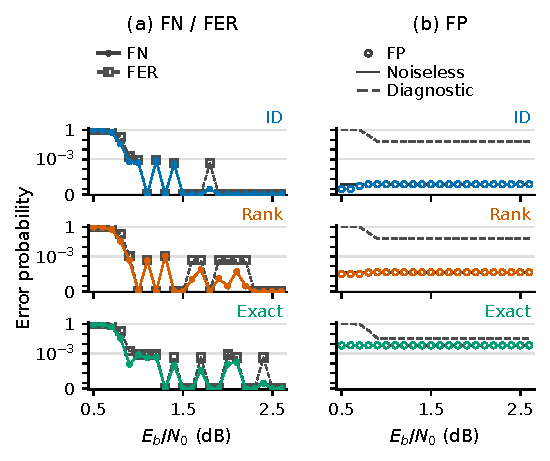
\includegraphics[width=\columnwidth]{itw2027/results/processed/figures/figure2_noisy.pdf}
  \caption{Packed BFC over AWGN: (a) channel-induced FN and payload FER; (b) conditional FP, paired noiseless reference, and empirical additive diagnostic.}
  \label{fig:itw27_noisy}
\end{figure}







\section{Conclusion}







\begin{thebibliography}{99}





\bibitem{beyond-bits}
D. G\"und\"uz, Z. Qin, I. E. Aguerri, H. S. Dhillon, Z. Yang, A. Yener, K.-K. Wong, and C.-B. Chae, ``Beyond transmitting bits: Context, semantics, and task-oriented communications,'' \emph{IEEE J. Sel. Areas Commun.}, vol. 41, no. 1, pp. 5--41, Jan. 2023.

\bibitem{task-oriented}
J. Shao, Y. Mao, and J. Zhang, ``Learning task-oriented communication for edge inference: An information bottleneck approach,'' \emph{IEEE J. Sel. Areas Commun.}, vol. 40, no. 1, pp. 197--211, Jan. 2022.

\bibitem{propositional-logic}
J. Bao, P. Basu, M. Dean, C. Partridge, A. Swami, W. Leland, and J. A. Hendler, ``Towards a theory of semantic communication,'' in \emph{Proc. IEEE Netw. Sci. Workshop (NSW)}, 2011, pp. 110--117.

\bibitem{BFC}
J. Zhu and M. Frey, ``Beyond identification: Computing Boolean functions via channels,'' in \emph{Proc. IEEE Int. Symp. Inf. Theory (ISIT)}, 2026, pp. 1--6.

\bibitem{ID}
R. Ahlswede and G. Dueck, ``Identification via channels,'' \emph{IEEE Trans. Inf. Theory}, vol. 35, no. 1, pp. 15--29, Jan. 1989.

\bibitem{ID-task}
Y. Zhao, H. Boche, and C. Deppe, ``Joint identification and sensing with noisy feedback: A task-oriented communication framework for 6G,'' arXiv:2603.29649, Mar. 2026.

\bibitem{BFC-capacity}
J. Zhu and M. Frey, ``Capacity regimes for Boolean function computation via channels,'' arXiv:2608.10816, Aug. 2026.

\bibitem{CWC}
S. Verd\'u and V. K. Wei, ``Explicit construction of optimal constant-weight codes for identification via channels,'' \emph{IEEE Trans. Inf. Theory}, vol. 39, no. 1, pp. 30--36, Jan. 1993.

\bibitem{RS-tagging}
P. Moulin and R. Koetter, ``A framework for the design of good watermark identification codes,'' in \emph{Proc. SPIE, Security, Steganography, Watermarking Multimedia Contents VIII}, vol. 6072, 2006.

\bibitem{RS-performance}
S. Derebeyo\u{g}lu, C. Deppe, and R. Ferrara, ``Performance analysis of identification codes,'' \emph{Entropy}, vol. 22, no. 10, Art.\ no. 1067, Oct. 2020.

\bibitem{RS-implementation}
R. Ferrara, L. Torres-Figueroa, H. Boche, C. Deppe, W. Labidi, U. J. M\"onich, and V. C. Andrei, ``Implementation and experimental evaluation of Reed--Solomon identification,'' in \emph{Proc. 27th Eur. Wireless Conf. (EW)}, 2022, pp. 7--12.

\bibitem{ID-tutorial}
C. von Lengerke, J. A. Cabrera, M. Reisslein, and F. H. P. Fitzek, ``Codes for identification via channels: Tutorial for communications generalists,'' \emph{IEEE Commun. Surveys Tuts.}, vol. 28, no. 1, pp. 181--223, Jan. 2026.


\bibitem{RS-code}
R. M. Roth, \emph{Introduction to Coding Theory}. Cambridge, U.K.: Cambridge Univ. Press, 2006.




\end{thebibliography}
